% !TEX root = ../presentation.tex
% Title

{
\setbeamertemplate{footline}[text line]{}

\usebackgroundtemplate{%
  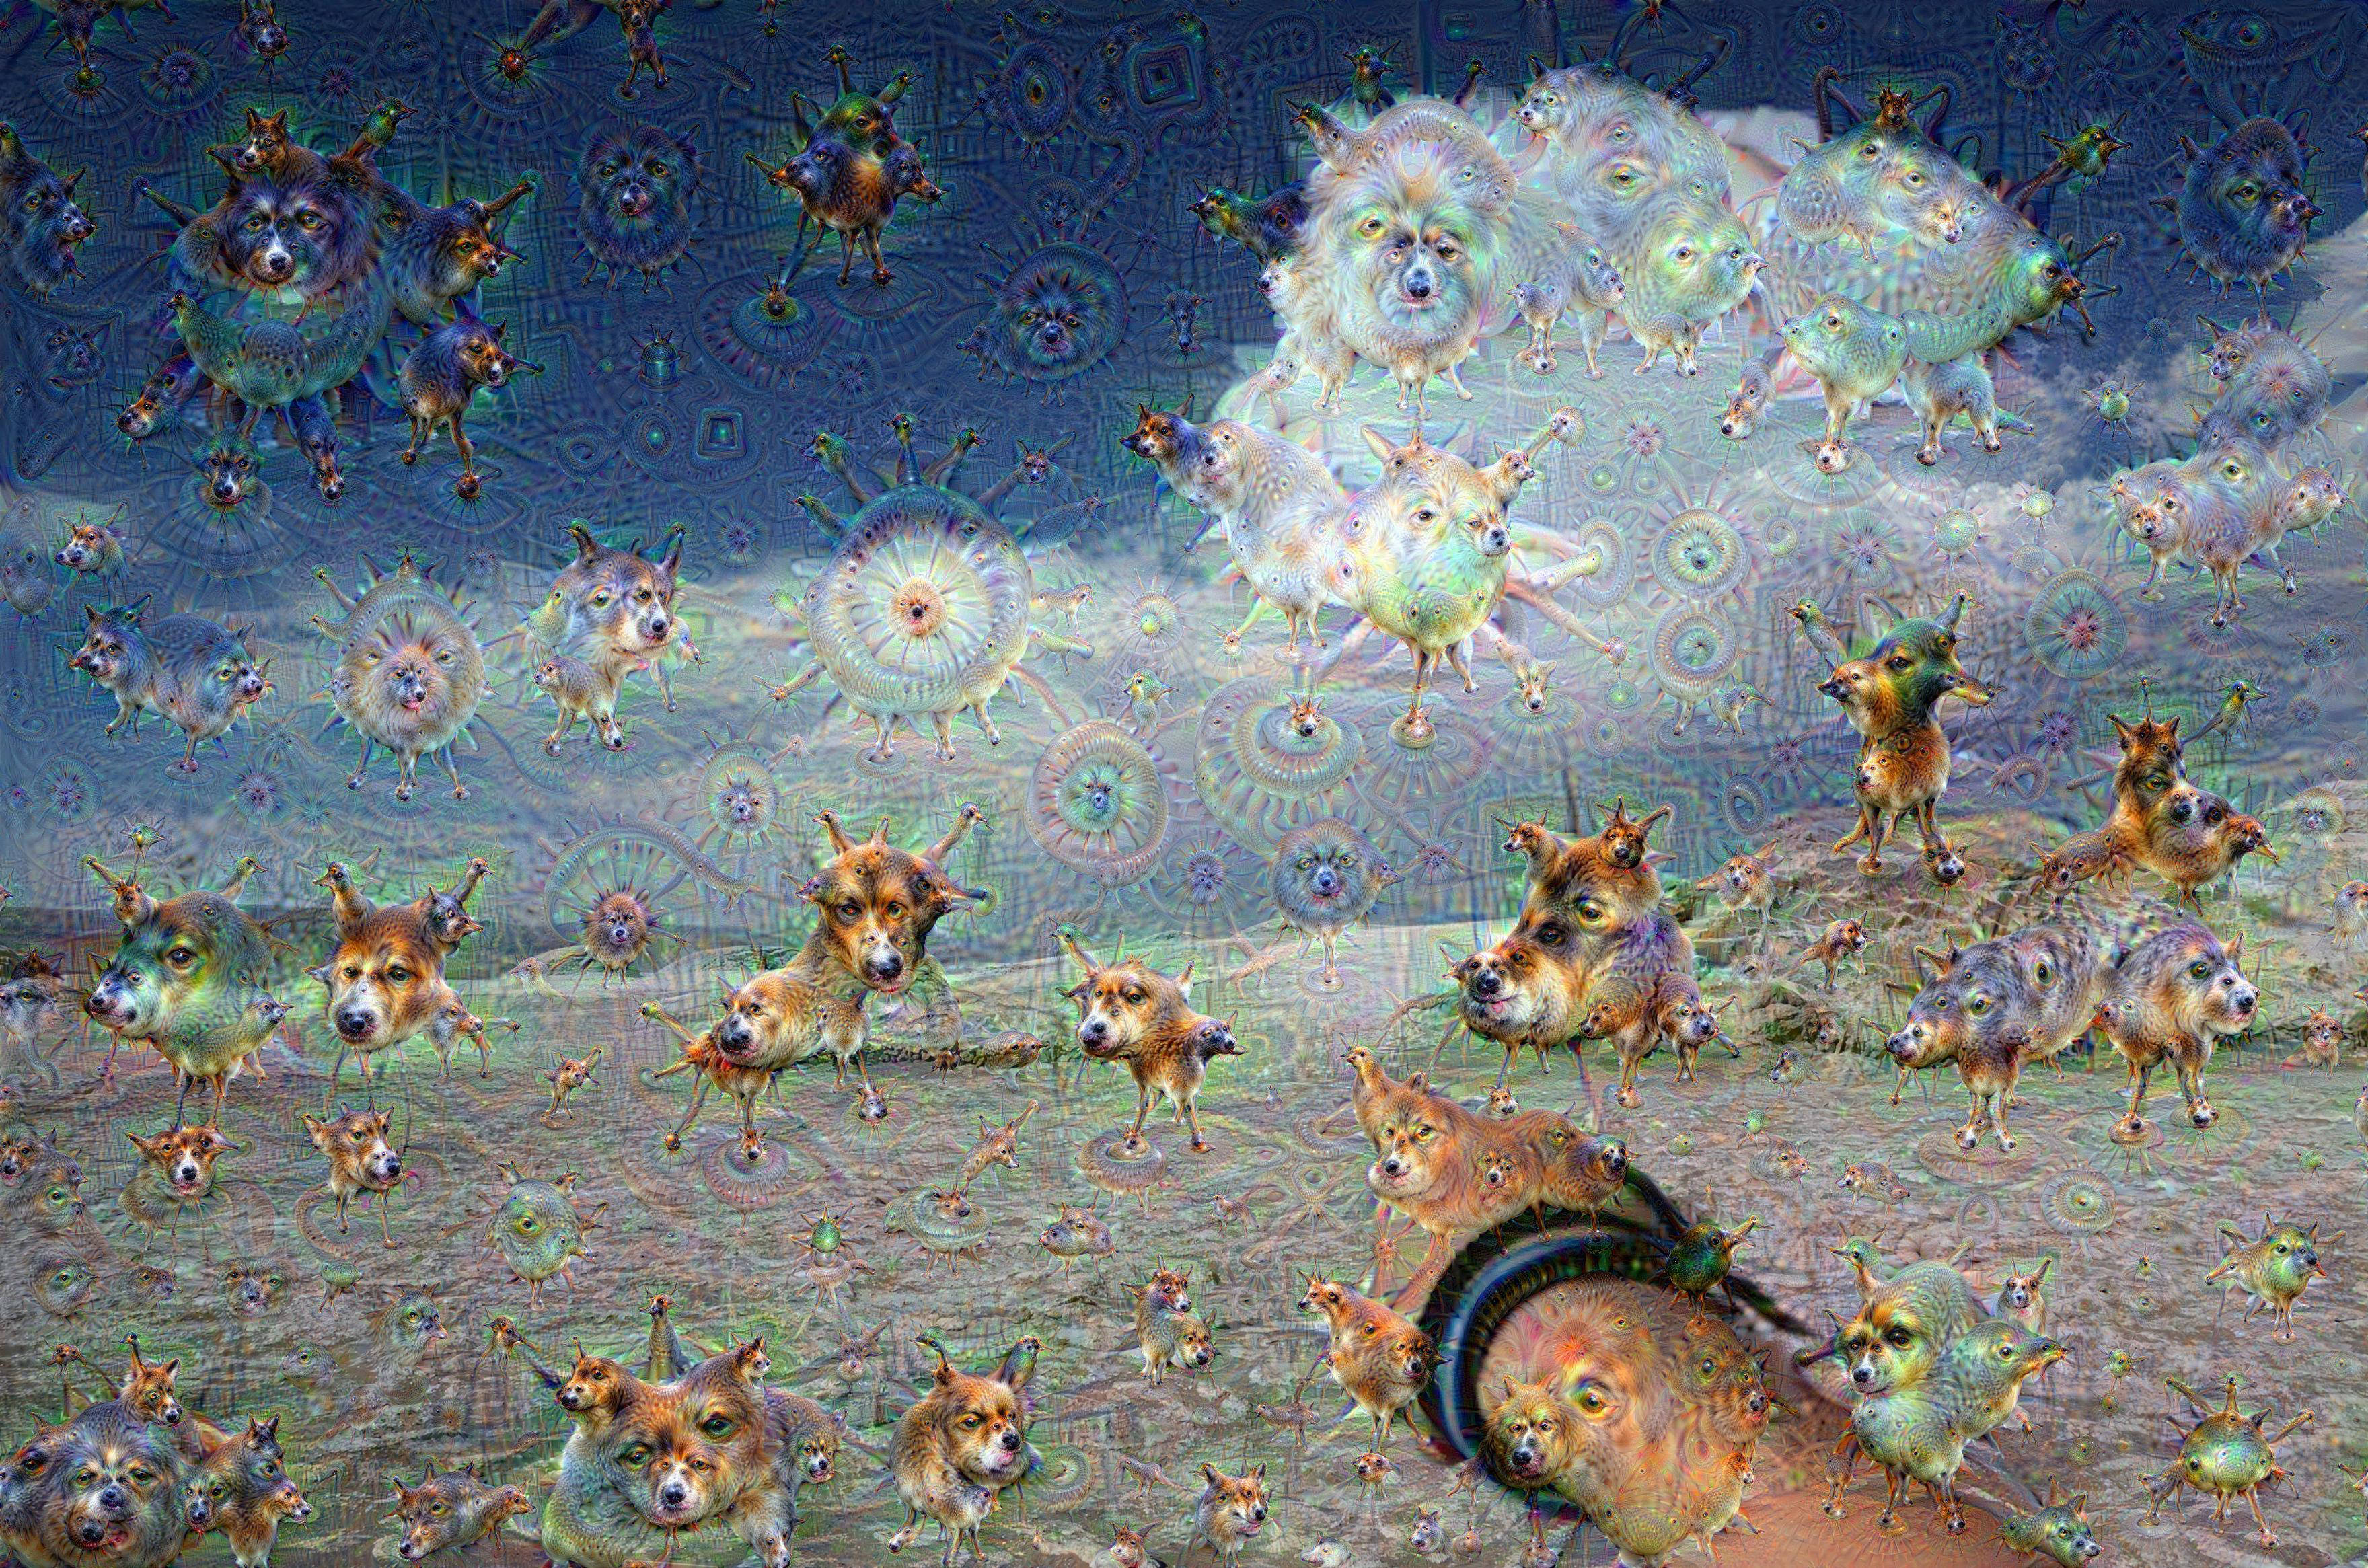
\includegraphics[width=\paperwidth,height=\paperheight]{deepdream}}
\begin{frame}
  \centering
  \vspace{2.28cm}
  \title
  {\begin{tcolorbox}[%
      colframe=black,%
      colback=black,%
      opacityframe=0,%
      opacityback=0.5,%
      boxrule=0.5pt,%
      arc=3pt,
      width=10cm]
    \centering
    \color{fb!10}
    {\large Engineering Challenges of Deep Learning} \\
    \vspace{-0.1cm}
    {\small feat. C++} \\
  \end{tcolorbox}

  \vspace{0.05cm}
  \begin{tcolorbox}[%
      colframe=black,%
      colback=black,%
      opacityframe=0,%
      opacityback=0.5,%
      boxrule=0.5pt,%
      arc=3pt,
      width=6cm]
      \centering
      \color{fb!10}
    {\small Peter Goldsborough}\\
    \vspace{-0.2cm}
    {\scriptsize Facebook}\\
    \vspace{-0.2cm}
    {\tiny \today}
  \end{tcolorbox}
  }
  \date{}
  \titlepage
\end{frame}
}

\usebackgroundtemplate{}

\addtocounter{framenumber}{-1}
